\documentclass[11pt]{article}

\usepackage{mathtools}
\usepackage{float}
\usepackage{amssymb}
\usepackage{amsmath}
\usepackage{amsthm}
\usepackage{hyperref}
\usepackage{microtype}
\usepackage{graphicx}
\usepackage{blkarray}
\usepackage{pgfplots}
\pgfplotsset{compat=1.15}
\usepackage{mathrsfs}
\usetikzlibrary{arrows}
\graphicspath{ {./img/} }

\setlength{\parindent}{0cm}
\let\emptyset\varnothing

\title{\textbf{MATH 2135 Linear Algebra} \\ Chapter 6 Inner Product Spaces}
\author{Alyssa Motas}

\begin{document}

    \maketitle

    \pagebreak

    \tableofcontents

    \pagebreak

    \section{6.A Inner Products and Norms}

    To motivate the concept of inner product, think of vectors in \(\mathbb{R}^2\) and \(\mathbb{R}^3\) as arrows with initial point at the origin. The length of a vector $x$ in \(\mathbb{R}^2\) or \(\mathbb{R}^3\) is called the \text{\emph{norm}} of $x$, denoted \(||x||\). Thus for \(x = (x_1, x_2) \in \mathbb{R}^2\), we have \(||x|| = \sqrt{x_1^2 + x_2^2}\). The generalization to \(\mathbb{R}^n\) is: we defined the norm of \(x = (x_1, \dots, x_n) \in \mathbb{R}^n \) by \[||x|| = \sqrt{x_1^2 + \dots + x_n^2.}\] 
    
    \begin{figure}[H]
        \centering
        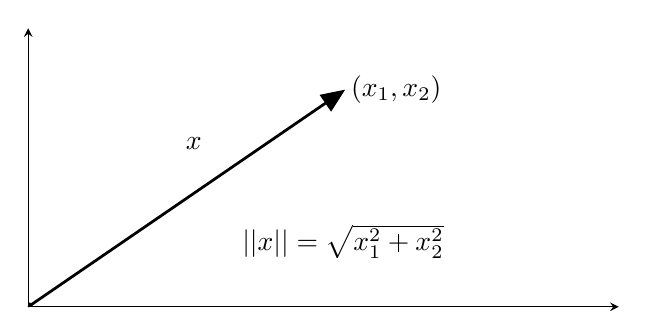
\begin{tikzpicture}[line cap=round,line join=round,>=triangle 45,x=1cm,y=1cm,scale=1]
            \begin{axis}[
            x=15cm,y=15cm,
            axis lines=middle,
            xmin=0,
            xmax=0.5,
            ymin=0,
            ymax=0.23585344119169532,
            ticks=none]
            \clip(-0.057132465392472714,-0.04075298644022664) rectangle (0.38291015883609275,0.23585344119169532);
            \draw [->,line width=1pt] (0,0) -- (0.2683348542861568,0.18381668611374563);
            \draw (0.12526118107302275,0.1517683147773752) node[anchor=north west] {$x$};
            \draw (0.2651441823780563,0.2039704573213492) node[anchor=north west] {$(x_1, x_2)$};
            \draw (0.1729420398340814,0.07787469228457479) node[anchor=north west] {$||x|| = \sqrt{x_1^2 + x_2^2}$};
            \begin{scriptsize}
            \draw [fill=black] (0,0) circle[radius=1.5pt];
            \end{scriptsize}
            \end{axis}
        \end{tikzpicture}
    \end{figure}
    
    The norm is not linear on \(\mathbb{R}^n\).

    \subsection{Definition of dot product}

    For \(x,y \in \mathbb{R}^n\), the \textbf{\emph{dot product}} of $x$ and $y$, denoted \(x \cdot y\), is defined by \[x \cdot y = x_1 y_1 + \dots + x_n y_n\] where \(x = (x_1, \dots, x_n)\) and \(y = (y_1, \dots, y_n)\). Note that the dot product of two vectors in \(\mathbb{R}^n\) is a number, not a vector. 

    \vspace{1em}

    An inner product is a generalization of the dot product. Recall that if \(\lambda = a + bi\), where \(a,b \in \mathbb{R}\), then 
    \begin{itemize}
        \item the absolute value of \(\lambda\), denoted \(|\lambda|\), is defined by \(|\lambda| = \sqrt{a^2 + b^2}\);
        \item the complex conjugate of \(\lambda\), denoted \(\overline{\lambda}\), is defined by \(\overline{\lambda} = a - bi\);
        \item \(|\lambda|^2 = \lambda \overline{\lambda}\).
    \end{itemize}
    For \(z = (z_1, \dots, z_n) \in \mathbb{C}^n\), we define the norm of $z$ by \[||z|| = \sqrt{|z_1|^2 + \dots + |z_n|^2}.\] The absolute values are needed because we want \(||z||\) to be nonegative number. Note that \[||z||^2 = z_1 \overline{z_1} + \dots + z_n \overline{z_n}.\] We want to think of \(||z||^2\) as the inner product of $z$ with itself. The equation above suggests that the inner product of \(w = (w_1, \dots, w_n) \in \mathbb{C}^n\) with $z$ should equal \[w_1 \overline{z_1} + \dots + w_n \overline{z_n}.\] If the roles of $w$ and $z$ were interchanged, the expression above would be its complex conjugate. We should expect that the inner product of $w$ with $z$ equals the complex conjugate of the inner product of $z$ with $w$. 

    \subsection{Definition of inner product}

    An \textbf{\emph{inner product}} on $V$ is a function that takes each ordered pair \((u,v)\) of elements of $V$ to a number \(\langle u,v \rangle \in \textbf{F}\) and has the following properties:

    \begin{enumerate}
        \item[] \textbf{positivity} \[\langle v,v \rangle \geq 0 \text{ for all } v \in V;\]
        \item[] \textbf{definiteness} \[\langle v,v \rangle = 0 \text{ if and only if } v = 0;\]
        \item[] \textbf{additivity in first slot} \[\langle u + v, w \rangle = \langle u,w \rangle + \langle v,w \rangle \text{ for all } u,v,w \in V;\]
        \item[] \textbf{homogeneity in first slot} \[\langle \lambda u, v \rangle = \lambda \langle u,v \rangle \text{ for all } \lambda \in \textbf{F} \text{ and all } u,v \in V;\]
        \item[] \textbf{conjugate symmetry} \[\langle u,v \rangle = \overline{\langle v,v \rangle} \text{ for all } u,v \in V.\]
    \end{enumerate}

    Every real number equals its complex conjugate. If we are dealing with a real vector space, then the last condition can be \(\langle u,v \rangle = \langle v,u \rangle\) for all \(v,w \in V\). 

    \subsubsection{Examples}
    \begin{enumerate}
        \item[(a)] The \textbf{\emph{Euclidean inner product}} on \(\textbf{F}^n\) is defined by \[\langle (w_1, \dots, w_n), (z_1, \dots, z_n) \rangle = w_1 \overline{z_1} + \dots + w_n \overline{z_n}.\]
        \item[(b)] If \(c_1, \dots, c_n\) are positive numbers, then an inner product can be defined on \(\textbf{F}^n\) by \[\langle (w_1, \dots, w_n), (z_1, \dots, z_n) \rangle = c_1 w_1 \overline{z_1} + \dots + c_n w_n \overline{z_n}.\]  
        \item[(c)] An inner product can be defined on the vector space of continuous real-valued functions on the interval \([-1,1]\) by \[\langle f,g \rangle = \int_{-1}^{1} f(x) \overline{g(x)}dx.\] This is an inner product since for example: additivity in the left slot is defined as
        \begin{align*}
            \langle f+h, g \rangle &= \int_{-1}^{1} (f(x) + h(x)) \overline{g(x)} dx \\
                                   &= \int_{-1}^{1} f(x) \overline{g(x)} + \int_{-1}^{1} h(x) \overline{g(x)} dx \\
                                   &= \langle f,g \rangle + \langle h,g \rangle.
        \end{align*} 
        \item[(d)] An inner product can be defined on \(\mathcal{P}(\mathbb{R})\) by \[\langle p,q \rangle = \int_{0}^{\infty} p(x) q(x) e^{-x} dx.\]  
        \item[(e)] The dot product on \(\mathbb{R}^n\) \[\langle v,w \rangle = v \cdot w = x_1 y_1 + \dots + x_n y_n\] and \[\langle v,v \rangle = v \cdot v = x_1^2 + \dots + x_n^2 \geq 0.\]
    \end{enumerate}

    \subsection{Definition of inner product space}

    An \textbf{\emph{inner product space}} is a vector space $V$ along with an inner product on $V$. For the rest of this chapter, $V$ denotes an inner product space over \textbf{F}. 

    \subsection{Basic properties of an inner product}

    \begin{enumerate}
        \item[(a)] For each fixed \(u \in V\), the function that takes $v$ to \(\langle v,u \rangle\) is a linear map from $V$ to \textbf{F}.
        \begin{proof}
            \begin{itemize}
                \item \(f(v+v') = \langle v+ v', u \rangle = \langle v,u \rangle + \langle v', u \rangle = f(v) + f(v')\)
                \item \(f(\lambda v) = \dots = \lambda f(v).\)
            \end{itemize}
        \end{proof} 
        \item[(b)] \(\langle 0,u \rangle = 0\) for every \(u \in V\).
        \item[(c)] \(\langle u,0 \rangle = 0\) for every \(u \in V\).
        \item[(d)] \(\langle u,v+w \rangle = \langle u,v \rangle + \langle u,w \rangle\) for all \(u,v,w \in V\).  
        \begin{proof}
            This is additivity in the second slot.
            \begin{align*}
                \langle u,v+w \rangle &= \overline{\langle v+w, u \rangle} \\
                                      &= \overline{\langle v,u \rangle + \langle w, u \rangle} \\
                                      &= \overline{\langle v,u \rangle} + \overline{\langle w,u \rangle} \\
                                      &= \langle u,v \rangle + \langle u,w \rangle. 
            \end{align*}
        \end{proof} 
        \item[(e)] \(\langle u, \lambda v \rangle = \overline{\lambda} \langle u,v \rangle\) for all \(\lambda \in \textbf{F}\) and \(u,v \in V\).  
        \begin{proof}
            This is homogeneity in the second slot.
            \begin{align*}
                \langle u, \lambda v \rangle &= \overline{\langle \lambda v, u \rangle} \\
                                             &= \overline{\lambda \langle v,u \rangle} \\
                                             &= \overline{\lambda} \overline{\langle v, u \rangle} \\
                                             &= \overline{\lambda} \langle u,v \rangle. 
            \end{align*}
        \end{proof} 
    \end{enumerate}

    \subsection{Definition of norm, \(||v||\)}

    For \(v \in V\), the \textbf{\emph{norm}} of $v$, denoted \(||v||\), is defined by \[||v|| = \sqrt{\langle v,v \rangle} \geq 0.\] Note that \(||v||^2 = \langle v,v \rangle.\)

    \subsection{Basic properties of the norm}

    Suppose \(v \in V\).

    \begin{enumerate}
        \item[(a)] \(||v|| = 0\) if and only if \(v = 0\). 
        \item[(b)] \(||\lambda v|| = |\lambda | ||v||\) for all \(\lambda \in \textbf{F}\).  
    \end{enumerate}
    \begin{proof}
        \begin{enumerate}
            \item[(a)] The desired result holds because \(\langle v,v \rangle = 0\) if and only if \(v = 0\).
            \item[(b)] Suppose \(\lambda \in \textbf{F}\). then
            \begin{align*}
                ||\lambda v||^2 &= \langle \lambda v, \lambda v \rangle \\
                                &= \lambda \langle v, \lambda v \rangle \\
                                &= \lambda \overline{\lambda} \langle v,v \rangle \\
                                &= |\lambda|^2 || v || 2.
            \end{align*}   
            Taking square roots now gives the desired equality. 
        \end{enumerate}
    \end{proof}

    \subsection{Definition of orthogonal}

    Two vectors \(u,v \in V\) are called \textbf{\emph{orthogonal}} if \(\langle u,v \rangle = 0\). We write \(u \perp v\) to mean ``$u$ is orthogonal to $v$.''

    \subsection{Orthogonality and 0}
    \begin{enumerate}
        \item[(a)] 0 is orthogonal to every vector in $V$.
        \item[(b)] 0 is the only vector in $V$ that is orthogonal to itself. 
        \begin{proof}
            If \(v \in V\) and \(\langle v,v \rangle = 0\), then \(v = 0\) (by definition of inner product).
        \end{proof}   
        \item[(c)] \(u \perp v \Leftrightarrow v \perp u\)
        \item[(d)] \(u \perp w\) and \(v \perp w \Rightarrow (u+v) \perp w\)  .
        \item[(e)] \(u \perp w\) and \(\lambda \in \textbf{F} \Rightarrow (\lambda u) \perp w\).   
    \end{enumerate}

    The last two properties imply that the set \[w^{\perp} = \{v \mid v \perp w\}\] is a subspace of $V$, called the \emph{orthogonal complement of $V$}.

    \begin{figure}[H]
        \centering
        \definecolor{qqqqff}{rgb}{0,0,1}
        \definecolor{ccqqqq}{rgb}{0.8,0,0}
        \begin{tikzpicture}[line cap=round,line join=round,>=triangle 45,x=1cm,y=1cm, scale=1]
        \clip(-2.6180510577677225,-0.020004894937517982) rectangle (13.737835166148363,10.261142907693804);
        \draw [line width=1pt,color=ccqqqq] (2.0820772765971225,5.817064550395381)-- (4.541491327323378,1.9614141749671257);
        \draw [line width=1pt,color=ccqqqq] (4.541491327323378,1.9614141749671257)-- (7.0585367634417295,3.566131921468393);
        \draw [line width=1pt,color=ccqqqq] (7.0585367634417295,3.566131921468393)-- (4.672005783374561,7.145928391569146);
        \draw [line width=1pt,color=ccqqqq] (4.672005783374561,7.145928391569146)-- (2.0820772765971225,5.817064550395381);
        \draw [->,line width=1pt] (0.7180503154458768,2.7986640315826374) -- (7.374186675539191,6.105800965213908);
        \draw [->,line width=1pt] (1.2343543936921086,6.8035091790601685) -- (8.574244803354755,1.724193382259398);
        \draw [->,line width=1pt] (4.387995520277201,0.5241352544438309) -- (4.429858013107976,9.775746170045235);
        \draw [->,line width=1pt,color=ccqqqq] (4.354489862439656,4.605448460592127) -- (3.950679670128945,5.954629104885521);
        \draw [->,line width=1pt,color=ccqqqq] (4.354489862439656,4.605448460592127) -- (4.99907668567554,5.7050107678506174);
        \draw [->,line width=1pt,color=ccqqqq] (4.354489862439656,4.605448460592127) -- (5.38848129144999,4.536796950527268);
        \draw [->,line width=1pt,color=ccqqqq] (4.354489862439656,4.605448460592127) -- (4.789397282566221,3.5582930693504466);
        \draw [->,line width=1pt,color=ccqqqq] (4.354489862439656,4.605448460592127) -- (4.060511738424303,3.7080640715713886);
        \draw [->,line width=1pt,color=ccqqqq] (4.354489862439656,4.605448460592127) -- (3.251748326431215,4.8163694880063606);
        \draw [->,line width=1pt,color=qqqqff] (4.354489862439656,4.605448460592127) -- (7.215687518545484,7.352491792280982);
        \draw (6.917544928186012,7.794948574975387) node[anchor=north west] {$\text{\color{blue} w}$};
        \draw (2.7485008127164028,7.167901937275228) node[anchor=north west] {$\text{\color{red} $w^{\perp}$}$};
        \end{tikzpicture}
    \end{figure}

    \subsection{Pythagorean Theorem}

    Suppose $u$ and $v$ are orthogonal vectors in $V$. Then \[||u+v||^2 = ||u||^2 + ||v||^2.\]
    \begin{proof}
        We have
        \begin{align*}
            ||u+v||^2 &= \langle u+v, u+v \rangle \\
                      &= \langle u, u+v \rangle + \langle v, u+v \rangle \\
                      &= \langle u, u \rangle + \underbrace{\langle u,v \rangle + \langle v,u \rangle}_{0} + \langle v,v \rangle \\
                      &= \langle u,u \rangle + \langle v,v \rangle \\
                      &= ||u||^2 + ||v||^2,
        \end{align*}
        as desired.
    \end{proof}

    \subsection{Orthogonal Decomposition (Projection)}

    Given \(u,v \in V\), assuming \(v \neq 0\). Then we can write $u$ as a sum of two vectors, the first of which is parallel to $v$ and the second is orthogonal to $v$.

    \begin{figure}[H]
        \centering
        \definecolor{ccqqqq}{rgb}{0.8,0,0}
        \definecolor{qqqqff}{rgb}{0,0,1}
        \begin{tikzpicture}[line cap=round,line join=round,>=triangle 45,x=1cm,y=1cm,scale=1.5]
        \clip(0.4659165179786193,4.826312037466861) rectangle (6.3117730368156115,8.500959444542582);
        \draw [->,line width=1pt,color=qqqqff] (1.7151488232431262,5.751036310032376) -- (3.15785216765511,5.745073864066619);
        \draw [->,line width=1pt,color=qqqqff] (1.7151488232431262,5.751036310032376) -- (3.94,8.09151);
        \draw [->,line width=1pt,color=ccqqqq] (1.7151488232431262,5.751036310032376) -- (3.94178,5.75);
        \draw [->,line width=1pt,color=ccqqqq] (3.94178,5.75) -- (3.94,8.09151);
        \draw (2.350938136976971,5.665795349571387) node[anchor=north west] {$\text{\color{blue} $v$}$};
        \draw (2.438702301424262,7.18831281107005) node[anchor=north west] {$\text{\color{blue}$u$}$};
        \draw (3.1751581161341447,5.620005350729322) node[anchor=north west] {$\text{\color{red} $cv$}$};
        \draw (4.167274757712224,6.947915317149209) node[anchor=north west] {$\text{\color{red} $w$}$};
        \end{tikzpicture}
    \end{figure}

    Let \(c = \dfrac{\langle u,v \rangle}{||v||^2} = \dfrac{\langle u,v \rangle}{\langle v,v \rangle}\) and let \(w = u - cv\). Then \(\langle w,v \rangle = 0\) and \(u = cv + w\). 

    \begin{proof}
        We know \(u = cv + w\) holds by the definition of $w$. We also know that $cv$ is parallel to $v$ by the definition of ``parallel.'' To prove that $w$ is orthogonal to $v$, we can calculate:
        \begin{align*}
            \langle w,v \rangle &= \langle u-cv, v \rangle \\
                                &= \langle u,v \rangle - c \langle v,v \rangle \\
                                &= \langle u,v \rangle - \frac{\langle u,v \rangle}{\langle v,v \rangle} \langle v,v \rangle \\
                                &= \langle u,v \rangle - \langle u,v \rangle = 0.
        \end{align*}
        Therefore, \(w \perp v.\)
    \end{proof}

    \subsection{Cauchy-Schwarz Inequality}

    Suppose \(u,v \in V\). Then \[|\langle u,v \rangle| \leq ||u|| ||v||.\] This inequality is an equality if and only if one of $u,v$ is a scalar multiple of the other. 
    \begin{proof}
        Consider two cases:

        \vspace{1em}
        
        \emph{Case 1.} \(v = 0\) and in this case, \(\langle u,v \rangle = 0, ||u|| \cdot ||v|| = || u || \cdot 0 = 0.\) So the inequality holds.

        \vspace{1em}

        \emph{Case 2.} \(v \neq 0\). Consider the orthogonal decomposition \[u = cv + w\] where \(c = \dfrac{\langle u,v \rangle}{\langle v,v \rangle}\) and \(w = u - cv\). We know that \(w \perp v\). By Pythagoras' Theorem,
        \begin{align*}
            ||u||^2 &= ||cv||^2 + ||w||^2 \\
                    \geq& ||cv||^2 \\
                    &= |c|^2 ||v||^2 \\
                    &= \bigg|\frac{\langle u,v \rangle}{||v||^2}\bigg|^2 ||v||^2 \\
                    &= \frac{| \langle u,v \rangle |^2}{||v||^4} \cdot ||v||^2 \\
                    &= \frac{|\langle u,v \rangle|^2}{||v||^2}.
        \end{align*}
        We just proved that \[||u||^2 \geq \frac{| \langle u,v \rangle|^2}{||v||^2}.\] Multiply both sides of the equation by \(||v||^2\) and we get \[||u||^2 ||v||^2 \geq | \langle u,v \rangle |^2.\] Take the square root of both sides of the equation and we get \[||u|| \cdot ||v|| \geq | \langle u,v \rangle |\] which is the Cauchy-Schwarz inequality. 
    \end{proof}

    \subsubsection{Examples of the Cauchy-Schawrz Inequality}

    \begin{enumerate}
        \item[(a)] If \(x_1, \dots, x_n, y_1, \dots, y_n \in \mathbb{R}\) then \[|x_1 y_1 + \dots + x_n y_n|^2 \leq (x_1^2 + \dots + x_n^2)(y_1^2 + \dots + y_n^2).\] 
        \item[(b)] If $f,g$ are continuous real-valued functions on \([-1,1]\), then \[\bigg| \int_{-1}^{1} f(x)g(x)dx \bigg|^2 \leq \left( \int_{-1}^{1} (f(x))^2 dx \right) \left( \int_{-1}^{1} (g(x))^2 dx \right).\] 
    \end{enumerate}

    \subsection{Triangle Inequality}

    The Triangle Inequality implies that the shortest path between two points is a line segment. Suppose \(u,v \in V\). Then \[||u+v|| \leq ||u|| + ||v||.\] This inequality is an equality if and only if one of $u,v$ is a nonnegative multiple of the other.

    \begin{figure}[H]
        \centering
        \definecolor{qqqqff}{rgb}{0,0,1}
        \begin{tikzpicture}[line cap=round,line join=round,>=triangle 45,x=1cm,y=1cm,scale=1.5]
        \clip(1.1158324500362908,6.0266553337393765) rectangle (4.326145012145141,8.04462595861587);
        \draw [->,line width=1pt,color=qqqqff] (1.48474,6.54) -- (3.5338464403969887,7.779766962780057);
        \draw [->,line width=1pt,color=qqqqff] (1.48474,6.54) -- (2.8660756239502043,6.543436994044301);
        \draw [->,line width=1pt,color=qqqqff] (2.8660756239502043,6.543436994044301) -- (3.5338464403969887,7.779766962780057);
        \draw (2.0923374460824555,6.437374173278102) node[anchor=north west] {$u$};
        \draw (3.3559265289490594,7.080693988269881) node[anchor=north west] {$v$};
        \draw (2.1033991731005815,7.724356690741059) node[anchor=north west] {$u+v$};
        \end{tikzpicture}
    \end{figure}

    \begin{proof}
        We have 
        \begin{align*}
            ||u+v||^2 &= \langle u+v, u+v \rangle \\
                      &= \langle u,u \rangle + \langle u,v \rangle + \langle v,u \rangle + \langle v,v \rangle \\
                      &= \langle u,u \rangle + \langle u,v \rangle + \overline{\langle u,v \rangle} + \langle v,v \rangle \\
                      &\leq \langle u,u \rangle + 2 |\langle u,v \rangle| + \langle v,v \rangle \\
                      &\leq \langle u,u \rangle + 2 ||u|| ||v|| + \langle v,v \rangle \quad (\text{Cauchy-Schwarz}) \\
                      &= ||u||^2 + 2 ||u|| ||v|| + ||v||^2 \\
                      &= (||u|| + ||v||)^2
        \end{align*}
        Taking the square roots: \[|| u+v|| \leq ||u|| + ||v||,\] thus we get the triangle inequality.
    \end{proof}

    \subsection{Parallelogram Equality}
    
    In every parallelogram, the sum of the squares of the lengths of the diagonals equals the sum of the squares of the lengths of the four sides.

    Suppose $u,v \in V$. Then \[||u+v||^2 + ||u - v||^2 = 2(||u||^2 + ||v||^2).\]

    \begin{figure}[H]
        \centering
        \definecolor{qqqqff}{rgb}{0,0,1}
        \begin{tikzpicture}[line cap=round,line join=round,>=triangle 45,x=1cm,y=1cm, scale=5]
        \clip(1.4054755144183175,6.3261733476284885) rectangle (3.805268705098164,7.634659537331268);
        \draw [->,line width=1pt,color=qqqqff] (1.712547506177378,6.697110503175739) -- (2.9356517789417698,6.783031051262492);
        \draw [->,line width=1pt,color=qqqqff] (1.712547506177378,6.697110503175739) -- (3.0973845753403673,7.543680609324636);
        \draw [->,line width=1pt,color=qqqqff] (1.712547506177378,6.697110503175739) -- (1.9955798998749232,7.392056112700953);
        \draw [->,line width=1pt,color=qqqqff] (1.9955798998749232,7.392056112700953) -- (2.9356517789417698,6.783031051262492);
        \draw [->,line width=1pt,color=qqqqff] (2.9356517789417698,6.783031051262492) -- (3.0973845753403673,7.543680609324636);
        \draw [->,line width=1pt,color=qqqqff] (1.9955798998749232,7.392056112700953) -- (3.0973845753403673,7.543680609324636);
        \draw (2.2654536225666435,6.6692247241029525) node[anchor=north west] {$u$};
        \draw (2.2638871779252074,6.969982095258647) node[anchor=north west] {$u+v$};
        \draw (1.709365774856888,7.140724561175161) node[anchor=north west] {$v$};
        \draw (2.29364962611249,7.35532747705188) node[anchor=north west] {$u-v$};
        \draw (3.098802171810559,7.1814521218524945) node[anchor=north west] {$v$};
        \draw (2.4628256473875707,7.599692841115882) node[anchor=north west] {$u$};
        \end{tikzpicture}
    \end{figure}

    \begin{proof}
        We have 
        \begin{align*}
            ||u+v||^2 + ||u-v||^2 &= \langle u+v, u+v \rangle + \langle u-v, u-v \rangle \\
                                  &= ||u||^2 + ||v||^2 + \langle u,v \rangle + \langle v,u \rangle \\
                                  &\quad + ||u||^2 + ||v||^2 - \langle u,v \rangle - \langle v,u \rangle \\
                                  &= 2(||u||^2 + ||v||^2),
        \end{align*}
        as desired.
    \end{proof}

    \section{6.B Orthonormal Bases}

    \section{6.C Orthogonal Complements and Minimization Problems}

\end{document}